\documentclass[a4paper]{article}

\def\npart {III}
\def\nterm {Michaelmas}
\def\nyear {2017}
\def\nlecturer {C.\ P.\ Caulfield}
\def\ncourse {Hydrodynamic Stability}

% Imports
\ifx \nextra \undefined
  \usepackage[pdftex,
    hidelinks,
    pdfauthor={Dexter Chua},
    pdfsubject={Cambridge Maths Notes: Part \npart\ - \ncourse},
    pdftitle={Part \npart\ - \ncourse},
  pdfkeywords={Cambridge Mathematics Maths Math \npart\ \nterm\ \nyear\ \ncourse}]{hyperref}
  \title{Part \npart\ - \ncourse}
\else
  \usepackage[pdftex,
    hidelinks,
    pdfauthor={Dexter Chua},
    pdfsubject={Cambridge Maths Notes: Part \npart\ - \ncourse\ (\nextra)},
    pdftitle={Part \npart\ - \ncourse\ (\nextra)},
  pdfkeywords={Cambridge Mathematics Maths Math \npart\ \nterm\ \nyear\ \ncourse\ \nextra}]{hyperref}

  \title{Part \npart\ - \ncourse \\ {\Large \nextra}}
\fi

\author{Lectured by \nlecturer \\\small Notes taken by Dexter Chua}
\date{\nterm\ \nyear}

\usepackage{alltt}
\usepackage{amsfonts}
\usepackage{amsmath}
\usepackage{amssymb}
\usepackage{amsthm}
\usepackage{booktabs}
\usepackage{caption}
\usepackage{enumitem}
\usepackage{fancyhdr}
\usepackage{graphicx}
\usepackage{mathtools}
\usepackage{microtype}
\usepackage{multirow}
\usepackage{pdflscape}
\usepackage{pgfplots}
\usepackage{siunitx}
\usepackage{tabularx}
\usepackage{tikz}
\usepackage{tkz-euclide}
\usepackage[normalem]{ulem}
\usepackage[all]{xy}

\pgfplotsset{compat=1.12}

\pagestyle{fancyplain}
\lhead{\emph{\nouppercase{\leftmark}}}
\ifx \nextra \undefined
  \rhead{
    \ifnum\thepage=1
    \else
      \npart\ \ncourse
    \fi}
\else
  \rhead{
    \ifnum\thepage=1
    \else
      \npart\ \ncourse\ (\nextra)
    \fi}
\fi
\usetikzlibrary{arrows}
\usetikzlibrary{decorations.markings}
\usetikzlibrary{decorations.pathmorphing}
\usetikzlibrary{positioning}
\usetikzlibrary{fadings}
\usetikzlibrary{intersections}
\usetikzlibrary{cd}

\newcommand*{\Cdot}{\raisebox{-0.25ex}{\scalebox{1.5}{$\cdot$}}}
\newcommand {\pd}[2][ ]{
  \ifx #1 { }
    \frac{\partial}{\partial #2}
  \else
    \frac{\partial^{#1}}{\partial #2^{#1}}
  \fi
}

% Theorems
\theoremstyle{definition}
\newtheorem*{aim}{Aim}
\newtheorem*{axiom}{Axiom}
\newtheorem*{claim}{Claim}
\newtheorem*{cor}{Corollary}
\newtheorem*{defi}{Definition}
\newtheorem*{eg}{Example}
\newtheorem*{fact}{Fact}
\newtheorem*{law}{Law}
\newtheorem*{lemma}{Lemma}
\newtheorem*{notation}{Notation}
\newtheorem*{prop}{Proposition}
\newtheorem*{thm}{Theorem}

\renewcommand{\labelitemi}{--}
\renewcommand{\labelitemii}{$\circ$}
\renewcommand{\labelenumi}{(\roman{*})}

\let\stdsection\section
\renewcommand\section{\newpage\stdsection}

% Strike through
\def\st{\bgroup \ULdepth=-.55ex \ULset}

% Maths symbols
\newcommand{\bra}{\langle}
\newcommand{\ket}{\rangle}

\newcommand{\N}{\mathbb{N}}
\newcommand{\Z}{\mathbb{Z}}
\newcommand{\Q}{\mathbb{Q}}
\renewcommand{\H}{\mathbb{H}}
\newcommand{\R}{\mathbb{R}}
\newcommand{\C}{\mathbb{C}}
\newcommand{\Prob}{\mathbb{P}}
\renewcommand{\P}{\mathbb{P}}
\newcommand{\E}{\mathbb{E}}
\newcommand{\F}{\mathbb{F}}
\newcommand{\cU}{\mathcal{U}}
\newcommand{\RP}{\mathbb{RP}}
\newcommand{\CP}{\mathbb{CP}}

\newcommand{\ph}{\,\cdot\,}

\DeclareMathOperator{\sech}{sech}
\DeclareMathOperator{\cosech}{cosech}
\DeclareMathOperator{\cosec}{cosec}

\DeclareMathOperator{\covol}{covol}
\DeclareMathOperator{\vol}{vol}

\let\Im\relax
\let\Re\relax
\DeclareMathOperator{\Im}{Im}
\DeclareMathOperator{\Re}{Re}
\DeclareMathOperator{\im}{im}
\DeclareMathOperator{\image}{image}
\DeclareMathOperator{\Ann}{Ann}

\DeclareMathOperator*{\res}{res}
\DeclareMathOperator{\Res}{Res}
\DeclareMathOperator{\Ind}{Ind}

\DeclareMathOperator{\tr}{tr}
\DeclareMathOperator{\diag}{diag}
\DeclareMathOperator{\rank}{rank}
\DeclareMathOperator{\card}{card}
\DeclareMathOperator{\spn}{span}
\DeclareMathOperator{\adj}{adj}

\DeclareMathOperator{\erf}{erf}
\DeclareMathOperator{\erfc}{erfc}

\DeclareMathOperator{\ord}{ord}
\DeclareMathOperator{\Sym}{Sym}

\DeclareMathOperator{\sgn}{sgn}
\DeclareMathOperator{\orb}{orb}
\DeclareMathOperator{\stab}{stab}
\DeclareMathOperator{\ccl}{ccl}

\DeclareMathOperator{\lcm}{lcm}
\DeclareMathOperator{\hcf}{hcf}

\DeclareMathOperator{\Int}{Int}
\DeclareMathOperator{\id}{id}

\DeclareMathOperator{\betaD}{beta}
\DeclareMathOperator{\gammaD}{gamma}
\DeclareMathOperator{\Poisson}{Poisson}
\DeclareMathOperator{\binomial}{binomial}
\DeclareMathOperator{\multinomial}{multinomial}
\DeclareMathOperator{\Bernoulli}{Bernoulli}
\DeclareMathOperator{\like}{like}

\DeclareMathOperator{\var}{var}
\DeclareMathOperator{\cov}{cov}
\DeclareMathOperator{\bias}{bias}
\DeclareMathOperator{\mse}{mse}
\DeclareMathOperator{\corr}{corr}

\DeclareMathOperator{\otp}{otp}
\DeclareMathOperator{\dom}{dom}

\DeclareMathOperator{\Root}{Root}
\DeclareMathOperator{\supp}{supp}
\DeclareMathOperator{\rel}{rel}
\DeclareMathOperator{\Hom}{Hom}
\DeclareMathOperator{\Aut}{Aut}
\DeclareMathOperator{\Gal}{Gal}
\DeclareMathOperator{\Mat}{Mat}
\DeclareMathOperator{\End}{End}
\DeclareMathOperator{\Char}{char}
\DeclareMathOperator{\ev}{ev}
\DeclareMathOperator{\St}{St}
\DeclareMathOperator{\Lk}{Lk}
\DeclareMathOperator{\disc}{disc}
\DeclareMathOperator{\Isom}{Isom}
\DeclareMathOperator{\length}{length}
\DeclareMathOperator{\energy}{energy}
\DeclareMathOperator{\area}{area}
\DeclareMathOperator{\Syl}{Syl}
\DeclareMathOperator{\cl}{cl}
\DeclareMathOperator{\fix}{fix}

\newcommand{\GL}{\mathrm{GL}}
\newcommand{\SL}{\mathrm{SL}}
\newcommand{\PGL}{\mathrm{PGL}}
\newcommand{\PSL}{\mathrm{PSL}}
\newcommand{\PSU}{\mathrm{PSU}}
\newcommand{\Or}{\mathrm{O}}
\newcommand{\SO}{\mathrm{SO}}
\newcommand{\U}{\mathrm{U}}
\newcommand{\SU}{\mathrm{SU}}

\renewcommand{\d}{\mathrm{d}}
\newcommand{\D}{\mathrm{D}}

\tikzset{->/.style = {decoration={markings,
                                  mark=at position 1 with {\arrow[scale=2]{latex'}}},
                      postaction={decorate}}}
\tikzset{<-/.style = {decoration={markings,
                                  mark=at position 0 with {\arrowreversed[scale=2]{latex'}}},
                      postaction={decorate}}}
\tikzset{<->/.style = {decoration={markings,
                                   mark=at position 0 with {\arrowreversed[scale=2]{latex'}},
                                   mark=at position 1 with {\arrow[scale=2]{latex'}}},
                       postaction={decorate}}}
\tikzset{->-/.style = {decoration={markings,
                                   mark=at position #1 with {\arrow[scale=2]{latex'}}},
                       postaction={decorate}}}
\tikzset{-<-/.style = {decoration={markings,
                                   mark=at position #1 with {\arrowreversed[scale=2]{latex'}}},
                       postaction={decorate}}}

\tikzset{circ/.style = {fill, circle, inner sep = 0, minimum size = 3}}
\tikzset{mstate/.style={circle, draw, blue, text=black, minimum width=0.7cm}}

\definecolor{mblue}{rgb}{0.2, 0.3, 0.8}
\definecolor{morange}{rgb}{1, 0.5, 0}
\definecolor{mgreen}{rgb}{0.1, 0.4, 0.2}
\definecolor{mred}{rgb}{0.5, 0, 0}

\def\drawcirculararc(#1,#2)(#3,#4)(#5,#6){%
    \pgfmathsetmacro\cA{(#1*#1+#2*#2-#3*#3-#4*#4)/2}%
    \pgfmathsetmacro\cB{(#1*#1+#2*#2-#5*#5-#6*#6)/2}%
    \pgfmathsetmacro\cy{(\cB*(#1-#3)-\cA*(#1-#5))/%
                        ((#2-#6)*(#1-#3)-(#2-#4)*(#1-#5))}%
    \pgfmathsetmacro\cx{(\cA-\cy*(#2-#4))/(#1-#3)}%
    \pgfmathsetmacro\cr{sqrt((#1-\cx)*(#1-\cx)+(#2-\cy)*(#2-\cy))}%
    \pgfmathsetmacro\cA{atan2(#2-\cy,#1-\cx)}%
    \pgfmathsetmacro\cB{atan2(#6-\cy,#5-\cx)}%
    \pgfmathparse{\cB<\cA}%
    \ifnum\pgfmathresult=1
        \pgfmathsetmacro\cB{\cB+360}%
    \fi
    \draw (#1,#2) arc (\cA:\cB:\cr);%
}
\newcommand\getCoord[3]{\newdimen{#1}\newdimen{#2}\pgfextractx{#1}{\pgfpointanchor{#3}{center}}\pgfextracty{#2}{\pgfpointanchor{#3}{center}}}

\def\Xint#1{\mathchoice
   {\XXint\displaystyle\textstyle{#1}}%
   {\XXint\textstyle\scriptstyle{#1}}%
   {\XXint\scriptstyle\scriptscriptstyle{#1}}%
   {\XXint\scriptscriptstyle\scriptscriptstyle{#1}}%
   \!\int}
\def\XXint#1#2#3{{\setbox0=\hbox{$#1{#2#3}{\int}$}
     \vcenter{\hbox{$#2#3$}}\kern-.5\wd0}}
\def\ddashint{\Xint=}
\def\dashint{\Xint-}


\begin{document}
\maketitle
{\small
\setlength{\parindent}{0em}
\setlength{\parskip}{1em}
Developing an understanding by which ``small'' perturbations grow, saturate and modify fluid flows is central to addressing many challenges of interest in fluid mechanics. Furthermore, many applied mathematical tools of much broader relevance have been developed to solve hydrodynamic stability problems, and hydrodynamic stability theory remains an exceptionally active area of research, with several exciting new developments being reported over the last few years.

In this course, an overview of some of these recent developments will be presented. After an introduction to the general concepts of flow instability, presenting a range of examples, the major content of this course will be focussed on the broad class of flow instabilities where velocity ``shear'' and fluid inertia play key dynamical roles. Such flows, typically characterised by sufficiently“high” Reynolds number $Ud/\nu$, where $U$ and $d$ are characteristic velocity and length scales of the flow, and $\nu$ is the kinematic viscosity of the fluid, are central to modelling flows in the environment and industry. They typically demonstrate the key role played by the redistribution of vorticity within the flow, and such vortical flow instabilities often trigger the complex, yet hugely important process of ``transition to turbulence''.

A hierarchy of mathematical approaches will be discussed to address a range of ``stability'' problems, from more traditional concepts of ``linear'' infinitesimal normal mode perturbation energy growth on laminar parallel shear flows to transient, inherently nonlinear perturbation growth of general measures of perturbation magnitude over finite time horizons where flow geometry and/or fluid properties play a dominant role. The course will also discuss in detail physical interpretations of the various flow instabilities considered, as well as the industrial and environmental application of the results of the presented mathematical analyses

\subsubsection*{Pre-requisites}
Elementary concepts from undergraduate real analysis. Some knowledge of complex analysis would be advantageous (e.g.\ the level of IB Complex Analysis/Methods). No knowledge of functional analysis is assumed.
}
\tableofcontents

\section{Instability of fluid at rest}
Recall that the Navier--Stokes equations for an incompressible fluid are
\[
  \rho\left(\frac{\partial \mathbf{u}}{\partial t} + \mathbf{u} \cdot \nabla \mathbf{u}\right) = - \nabla P- g \rho \hat{\mathbf{z}} + \mu \nabla^2 \mathbf{u},\quad \nabla \cdot \mathbf{u} = 0. 
\]
Usually, when doing fluid mechanics, we assume density is constant, and divide the whole equation across by $\rho$. We can then forget the existence of $\rho$ and carry on. We can also get rid of the gravity term. We know that the force of gravity is balanced out by a hydrostatic pressure gradient. More precisely, we can write
\[
  P = P_h(z) + p (x, t),
\]
where $P_h$ satisfies
\[
  \frac{\partial P_h}{\partial z} = -g\rho.
\]
We can then write our equation as
\[
  \frac{\partial \mathbf{u}}{\partial t} + \mathbf{u}\cdot \nabla \mathbf{u} = - \nabla \left(\frac{p}{\rho}\right) + \nu \nabla^2 \mathbf{u}.
\]
To do all of these, we must assume that the density $\rho$ is constant. This is not helpful if we want to study, say, the interface between two different liquids. Thus, we do not make this assumption.

Since it is rather difficult to move forward without making \emph{any} simplifying assumptions, we shall focus on the case of inviscid fluids, so that we take $\nu = 0$. We will also assume that the fluid is irrotational. In this case, it is convenient to use the vector calculus identity 
\[
  \mathbf{u} \cdot \nabla \mathbf{u} = \nabla \left(\frac{1}{2}|\mathbf{u}|^2\right) - \mathbf{u} \times (\nabla \times \mathbf{u}),
\]
where we can now drop the second term. Moreover, since $\nabla \times \mathbf{u} = 0$, Stokes' theorem allows us to write $\mathbf{u} = \nabla \phi$ for some \term{velocity potential} $\phi$. Finally, we make the simplifying assumption that $\nabla \rho$ is negligible in the regions we care about. Under all these assumptions, we have
\[
  \nabla \left(\rho \frac{\partial \phi}{\partial t} + \frac{1}{2} \rho |\nabla \phi|^2 + P + g \rho z\right) = 0.
\]
This is essentially the Bernoulli's theorem.

What we would like to do is to use this to study the interface between two fluids:
\begin{center}
  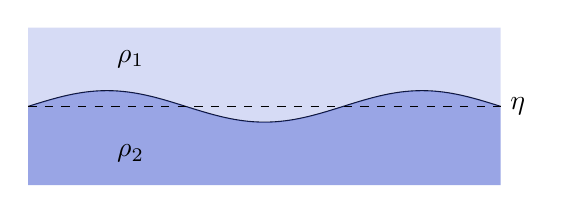
\begin{tikzpicture}
    \draw (-3, 0) sin (-2, 0.2) cos (-1, 0) sin (0, -0.2) cos (1, 0) sin (2, 0.2) cos (3, 0) node [right] {$\eta$};
    \fill [mblue, opacity=0.5] (-3, -1) -- (-3, 0) sin (-2, 0.2) cos (-1, 0) sin (0, -0.2) cos (1, 0) sin (2, 0.2) cos (3, 0) -- (3, -1);
    \fill [mblue, opacity=0.2] (-3, 1) -- (-3, 0) sin (-2, 0.2) cos (-1, 0) sin (0, -0.2) cos (1, 0) sin (2, 0.2) cos (3, 0) -- (3, 1);

    \draw [dashed] (-3, 0) -- (3, 0);
    \node at (-1.7, -0.6) {$\rho_2$};
    \node at (-1.7, 0.6) {$\rho_1$};
  \end{tikzpicture}
\end{center}

The model is that we start with a flat surface, with $\eta = 0$ and $\mathbf{u} = \mathbf{0}$. We then introduce some small perturbations of $\eta$, and see how the field responses.

For simplicity, assume there is no $y$ dependence. Let's figure out what equations we have. The incompressibility assumption tells us
\[
  \nabla^2 \phi = 0.
\]
We also assume that there is no velocity in the far field, i.e.\ $\phi_1 \to 0$ as $z \to \infty$ and $\phi_2 \to 0$ as $z \to-\infty$ (and similarly for the derivatives). This is a reasonable assumption to make if we only want to understand the behaviour of the interface.

We next need a \term{kinematic boundary condition}, telling us the vertical velocities of the fluids and the interface match:
\[
  \left.\frac{\partial \phi_{1, 2}}{\partial z} \right|_{z = \eta} = \frac{\D \eta}{\D t},
\]
where
\[
  \D = \frac{\partial}{\partial t} + \mathbf{u} \cdot \nabla
\]

Finally, we need to impose our actual equations of motion. We know the quantity 
\[
  \rho \frac{\partial \phi}{\partial t} + \frac{1}{2} \rho |\nabla \phi|^2 + P + g \rho z
\]
should be constant. Matching at the interface, we need
\[
  \left.\rho_1 \frac{\partial \phi_1}{\partial t} + \frac{1}{2} \rho_1 |\nabla \phi_1|^2 + P_1 + g \rho_1 \eta\right|_{z = \eta} = \left.\rho_2 \frac{\partial \phi_2}{\partial t} + \frac{2}{2} \rho_2 |\nabla \phi_2|^2 + P_2 + g \rho_2 \eta\right|_{z = \eta}.
\]
We need a physical assumption that the pressure is continuous along the interface. This does not always hold at all interfaces. For example, if we have a balloon, then the pressure inside is greater than the pressure outside, since that is what holds the balloon up. In this case, it is the rubber that is exerting a force to maintain the pressure difference. In our case, we only have two fluids meeting, and there is no reason to assume a discontinuity in pressure, and thus we shall assume it is continuous (we will revisit this assumption later on).

This assumption allows us to simplify our equation slightly into
\[
  \rho_1 \frac{\partial \phi_1}{\partial t} + \frac{1}{2} \rho_1 |\nabla \phi_1|^2 + g \rho_1 \eta = \rho_2 \frac{\partial \phi_2}{\partial t} + \frac{2}{2} \rho_2 |\nabla \phi_2|^2 + g \rho_2 \eta 
\]
These equations are pretty nasty and non-linear. At this point, one sensible approach is to linearize the equations by assuming everything is small. In addition to assuming that $\eta$ is small, we also need to assume that various derivatives such as $\nabla \phi$ are small, so that we can drop all second-order terms. We can also replace the evaluations at $\eta$ with evaluations at $z = 0$. We are then left with the collection of $3$ equations
\begin{align*}
  \nabla^2 \phi_{1, 2} &= 0\\
  \left.\frac{\partial \phi_{1, 2}}{\partial z}\right|_{z = 0} &= \eta_t\\
  \left.\rho_1 \frac{\partial \phi_1}{\partial t} + g \rho_1 \eta \right|_{z = 0} &= \left.\rho_2 \frac{\partial \phi_2}{\partial t} + g \rho_2 \eta \right|_{z = 0}
\end{align*}

We now have a nice linear problem. The plan is to analyze the Fourier modes of the solutions, plugging in an ansatz
\begin{align*}
  \phi_{1, 2}(x, z, t) &= \hat{\phi}_{1, 2}(z) e^{i(kx - \omega t)}\\
  \eta(x, t) &= B e^{i(kx - \omega t)}.
\end{align*}
Substituting into Laplace's equation gives
\[
  \hat{\phi}_{1, 2} - k^2 \hat{\phi}_{1, 2} = 0.
\]
Using the far field boundary conditions, we see that we have a family of solutions
\[
  \hat{\phi}_1 = A_1 e^{-kz},\quad \hat{\phi}_2 = A_2 e^{kz}.
\]
The kinematic boundary condition tells us we must have
\[
  \hat{\phi}_{1, 2}'(0) = -i\omega B.
\]
We can solve this to get
\[
  B = \frac{k A_1}{i \omega} = - \frac{kA_2}{ i \omega}.
\]
In particular, we must have $A \equiv A_1 = - A_2$. We can then write
\[
  \eta = \frac{kA}{i\omega} e^{ik(kx - \omega t)}.
\]
Plugging these into the final equation gives us
\[
  \rho_1 (-i\omega A) + g \rho_1 \frac{k A}{i \omega} = \rho_2 i \omega A + g \rho_2 \frac{kA}{i \omega}.
\]
Crucially, we can cancel the $A$ throughout the equation, and gives us a result independent of $A$. This is, after all, the point of linearization. Solving this gives us a \term{dispersion relation} relating the frequency (or phase speed $c_p = \omega/k$) to the wavenumber:
\[
  \omega^2 = \frac{g(\rho_2 - \rho_1)k}{\rho_1 + \rho_2}.
\]
If $\rho_2 \gg  \rho_1$, then this reduces to $\omega^2 \approx gk$, and this is the usual dispersion relation for deep water waves. On the other hand, if $\rho_2 - \rho_1 > 0$ is small, this can lead to waves of rather low frequency, which is something we can observe in cocktails, apparently.

But nothing in our analysis actually required $\rho_2 > \rho_1$. Suppose we had $\rho_1 > \rho_2$. This amounts to putting the heavier fluid on top of the lighter one. Anyone who has tried to turn a cup of water upside down will know this is highly unstable. Can we see this from our analysis?

If $\rho_1 < \rho_2$, then $\omega$ has to be imaginary. We shall write it as $\omega = \pm i \sigma$, where $\sigma > 0$. We can then compute
\[
  \sigma = \sqrt{\frac{g(\rho_1 - \rho_2)k}{\rho_1 + \rho_2}}.
\]
Writing out our expression for $\phi_{1, 2}$, we see that there are $e^{\pm \sigma t}$ terms, and the $e^{\sigma t}$ term dominates in the long run, causing $\phi_{1, 2}$ to grow exponentially. This is the \emph{Rayleigh--Taylor instability}.

There is more to say about the instability. As the wavelength decreases, $k$ increases, and we see that $\sigma$ increases as well. Thus, we see that short-scale perturbations blow up exponentially much more quickly, which means the system is not very well-posed. This is the \term{ultra-violet catastrophe}. Of course, we should not trust our model here. Recall that in our simplifying assumptions, we not only assumed that the amplitudes of our $\phi$ and $\eta$ were small, but also that their derivatives were small. The large $k$ behaviour gives us large $x$ derivatives, and so we have to take into account the higher order terms as well.

But we can also provide physical reasons for why small scales perturbations should be suppressed by such a system. In our model, we assumed there is no surface tension. Surface tension quantifies the tendency of interfaces between fluids to minimize surface area. We know that small-scale variations will cause a large surface area, and so the surface tension will suppress these variations. Mathematically, what the surface allows for is a pressure jump across the interface.

Surface tension is quantified by $\gamma$, the force per unit length. This has dimensions $[\gamma] = MT^{-1}$. Empirically, we observe that the pressure difference across the interface is
\[
  \Delta p = - \gamma \nabla \cdot \hat{\mathbf{n}} = 2 \gamma H = \gamma \left(\frac{1}{R_x} + \frac{1}{R_y}\right),
\]
where $\hat{\mathbf{n}}$ is the unit normal and $H$ is the \term{mean curvature}. This is an empirical result. 

Again, we assume no dependence in the $y$ direction, so we have a cylindrical interface with a single radius of curvature. Linearizing, we have a pressure difference of
\[
  (P_2 - P_1) |_{z = \eta} = \frac{\gamma}{R_x} = - \gamma \frac{\frac{\partial^2 \eta}{\partial x^2}}{\left(1 + \left(\frac{\partial \eta}{\partial x}\right)^2\right)^{3/2}} \approx -\gamma \frac{\partial^2 \eta}{\partial x^2}.
\]
Therefore the (linearized) dynamic boundary condition becomes
\[
  \left.\rho_1 \frac{\partial \phi_1}{\partial t} + g \rho_1 \eta\right|_{z =0 } + \gamma \frac{\partial^2 \eta}{\partial x^2} = \left. \rho_2 \frac{\partial \phi_2}{\partial t} + g \rho_2 \eta\right|_{z = 0}.
\]
If we run the previous analysis again, we find a dispersion relation of
\[
  \omega^2 = \frac{g(\rho_2 - \rho_1)k + \gamma k^3}{\rho_1 + \rho_2}.
\]
Since $\gamma$ is always positive, even if we are in the situation when $\rho_1 > \rho_2$, for $k$ sufficiently large, the system is stable. Of course, for small $k$, the system is still unstable --- we still expect water to fall out even with surface tension. In the case $\rho_1 < \rho_2$, what we get is known as \term{internal gravity-capillary waves}.

In the unstable case, we have
\[
  \sigma^2 = k \left(\frac{g(\rho_2 - \rho_1)}{\rho_1 + \rho_2}\right) (1 - l_c^2 k^2),
\]
where
\[
  l_c^2 = \frac{\gamma}{g (\rho_1 - \rho_2)}
\]
is a characteristic length scale. For $k \ell_c > 1$, the oscillations are stable, and the maximum value of $k$ is attained at $k = \frac{l_c}{\sqrt{3}}$.
% insert plot

In summary, we have a range of wavelength, and we have identified a ``most unstable wavelength''. Over time, if all frequencies modes are triggered, we should expect this most unstable wavelength to dominate. But it is rather hopeful thinking, because this is the result of linear analysis, and we can't expect it to carry on to the non-linear regime.

\subsection{Rayleigh--Benard convection}
We now want to study what happens when we genuinely have density variations throughout the fluid, and not just an interface between the two fluids. What we ultimately want to model is a fluid that with temperature variations, such as flow in the sea (though sea water is much more complicated since there are many other factors affecting the density, such as salinity). To do so, we need to assume that $\rho$ is genuinely varying.

%The set up of the Rayleigh--Benard convection is as follows --- we have a fluid that is cooled above and heated below. Thus, the fluid is less dense below and more dense above. Curiously, this set up is stable when the heating rate is low. However, as the heating rate increases, we see some rather beautiful structures appearing: 
%
% insert picture
%
%Later, it was realized that these patterns were not due to the temperature gradient itself, but the surface tension gradient.

Again, recall that the Navier--Stokes equation
\[
  \rho\left(\frac{\partial \mathbf{u}}{\partial t} + \mathbf{u} \cdot \nabla \mathbf{u}\right) = - \nabla P- g \rho \hat{\mathbf{z}} + \mu \nabla^2 \mathbf{u},\quad \nabla \cdot \mathbf{u} = 0. 
\]
To make our lives more pleasant, we decompose the density field into a horizontally (and temporally) averaged hydrostatic part and a perturbation part:
\[
  \rho = \rho_h(z) + \rho'(x, t).
\]
We can then define the hydrostatic pressure by the equation
\[
  \frac{\d P_h}{\d z} = - g\rho_h.
\]
This then allows us to decompose the pressure as
\[
  P = P_h(z) + p'(x, t).
\]
Then our equations of motion become
\[
  \frac{\partial u}{\partial t} + u \cdot u = - \frac{1}{\rho} \nabla p' - \frac{g\rho'}{\rho} \hat{\mathbf{z}} + \nu \nabla^2 \mathbf{u},\quad \nabla \cdot \mathbf{u} = 0
\]
We have effectively ``integrated out'' the hydrostatic part, and it is now the deviation from the average that leads to buoyancy forces.

When we have density variations, one interesting thing to look at is the vorticity. Returning to the case where we have an interface, if we just have a lighter fluid above a heavier fluid:
\begin{center}
  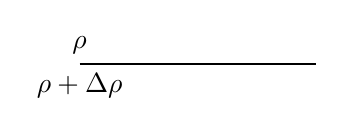
\begin{tikzpicture}
    \draw (0, 0) -- (3, 0);
    \node at (0, 0) [above] {$\rho$};
    \node at (0, 0) [below] {$\rho + \Delta \rho$};
  \end{tikzpicture}
\end{center}
If we have this, then nothing happens. But what if the interface is tilted? If it looks like this:
\begin{center}
  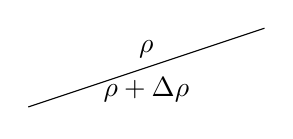
\begin{tikzpicture}
    \draw (0, 0) -- (3, 1);
    \node [above] at (1.5, 0.5) {$\rho$};
    \node [below] at (1.5, 0.5) {$\rho + \Delta \rho$};
  \end{tikzpicture}
\end{center}
then we expect there to be a tendency for the interface to return horizontal. The fluid to the left will move up, and the fluid to the right will move down. This gives rise to \emph{vorticity}.

Mathematically, the reason this happens is that the direction of the density gradient does not align with the direction of gravity. More precisely, this is because the density gradient does not align with the pressure gradient.

We can see this from our equations. Recall that the vorticity is defined by\index{vorticity}\index{$\boldsymbol\omega$}
\[
  \boldsymbol\omega = \nabla \times \mathbf{u}.
\]
Taking the curl of the Navier--Stokes equation, we obtain the equation.
\[
  \frac{\partial \boldsymbol\omega}{\partial t} + \mathbf{u} \cdot \nabla \boldsymbol\omega = \boldsymbol\omega \cdot \nabla \mathbf{u} + \frac{1}{\rho^2}\nabla \rho \times \nabla P + \nu \nabla^2 \boldsymbol\omega
\]
Let's interpret these terms one by one. The term on the left hand side is just the material derivative of the vorticity. So we should interpret the terms on the right-hand-side as the terms that contribute to the change in vorticity.

The first and last terms are familiar terms that have nothing to do with the density gradient. The interesting term is the second one. This is what we just described --- whenever the pressure gradient and density gradient do not align, we have a \term{baroclinic torque}. % describe other terms as well.

%The left hand side is just the change in vorticity along the flow. The first term on the left is describing what happens when we stretch a vortex, which by conservation of momentum implies that the spin increases. The second term is what we just described --- if the pressure gradient points differently from the density gradient, then we get a torque, called \term{baroclinic torque}.

In general, equations are hard to solve, and we want to make approximations. A common approximation is the \term{Boussinesq approximation}. The idea is that even though the density difference is often what drives the motion, from the point of inertia, the variation in density is often small enough to be ignored. To take some actual, physical examples, salt water is roughly $4\%$ more dense than fresh water, and every $10$ degrees Celsius changes the density of air by approximately $4\%$.

Thus, what we do is that we assume that the density is constant except in the buoyancy force. The mathematically inclined people could think of this as taking the limit $g \to \infty$ but $\rho' \to 0$ with $g \rho'$ remaining finite.

Under this approximation, we can write our equations as
\begin{align*}
  \frac{\partial \mathbf{u}}{\partial t} + \mathbf{u}\cdot \nabla \mathbf{u} &= - \frac{1}{\rho_0} \nabla p' - g' \hat{\mathbf{z}} + \nu \nabla^2 \mathbf{u}\\
  \frac{\partial \boldsymbol\omega}{\partial t} + \mathbf{u} \cdot \nabla\boldsymbol\omega &= \omega \cdot \nabla \mathbf{u} + \frac{g}{\rho_0} \hat{\mathbf{z}} \times \nabla \rho + \nu \nabla^2 \boldsymbol\omega,
\end{align*}
where we define
\[
  g' = \frac{g \rho'}{\rho_0}
\]
It is typically assumed that the kinematic viscosity is constant.

These equations are, of course, not enough to obtain a solution. We must have equations determining the density. In our models, our density will be a function of $T$, and in turn $T$ evolves via the diffusion equation
\[
  \frac{\partial T}{\partial t} + \mathbf{u} \cdot \nabla T = \kappa \nabla^2 T.
\]
In reality, the dependence of $\rho$ on $T$ may be extremely complicated, and moreover there may be other factors determining $\rho$. However, for our purposes, we will use a ``leading-order'' approximation
\[
  \rho = \rho_0 (1 - \alpha(T - T_0)).
\]
Note that we will completely forget about thermodynamics, and do not use thermodynamics to impose relations between temperature and pressure, say. In particular, pressure will not serve as a thermodynamic quantity. Its only purpose is to act as a non-local Lagrange multiplier that enforces incomrpessibility.

Let's think about matters more carefully. Usually, to derive incompressibility, we use the conservation of mass
\[
  \frac{\partial \rho}{\partial t} + \nabla \cdot (\mathbf{u} \rho) = 0,
\]
which expands to give
\[
  \frac{\partial \rho}{\partial t} + \mathbf{u} \cdot \nabla \rho = - \rho \nabla \cdot \mathbf{u}.
\]
If $\rho$ is constant, then the terms on the left drop out and we find that $\nabla \cdot \mathbf{u} = 0$. Here we might need to do ab it more work.

Since we expressed $\rho$ in terms of $T$, we need to know how $T$ changes. It satisfies the diffusion equation
\[
  \frac{\partial T}{\partial t} + \mathbf{u} \cdot \nabla T = \kappa \nabla^2 T.
\]
Expressing $T$ in terms of $\rho$ and $\rho_0$, this gives
\[
  -\frac{1}{\rho_0 \alpha} \left(\frac{\partial \rho}{\partial t} + \mathbf{u} \cdot \nabla \rho\right) = - \frac{\kappa}{\rho_0 \alpha} \nabla^2 \rho.
\]
So we find that we must have
\[
  \frac{\partial \rho}{\partial t} + \mathbf{u} \cdot \nabla \rho = \kappa \nabla^2 \rho.
\]
This seems to conflict with the conservation of mass. The way we should think about this is that we should think of the failure of incompressibility as a ``diffusion of density''.

% \frac{\partial T}{\partial t} + \mathbf{u} \cdot \nabla T = \kappa \nabla^2 T

% \frac{\partial \rho}{\partial t} + \mathbf{u} \cdot \nabla \rho = \kappa \nabla^2 \rho

% U = 0
% T_h = T_0 - \Delta T \frac{(z - d)}{d}
% \rho_h = \rho_0 \left(1 + \alpha \Delta T \frac{(z - d}{d}\right)
% P_h = P_0 - g \rho_0 \left(z + \frac{\alpha \Delta Tz}{2d}[z - 2d]\right)

% \mathbf{u} = \mathbf{U} + \mathbf{u}'
% T = T_h + \theta
% P = P_h + p'

% \frac{\partial \mathbf{u}}{\partial t} + \mathbf{u} \cdot \nabla \mathbf{u} = -\frac{1}{\rho_0} \nabla p' + g \alpha \theta \hat{\mathbf{z}} + \nu \nabla^2 \mathbf{u}
% \frac{\partial \mathbf{u}'}{\partial } = - \frac{1}{\rho_0} \nabla p' + g \alpha \theta \hat{\mathbf{z}} + \nu \nabla^2 \mathbf{u}
% \nabla \cdot \mathbf{u}' = 0

% \frac{\partial T}{\partial t} + \mathbf{u} \cdot \nabla T = \kappa \nabla^2 T
% \frac{\partial \theta}{\partial t} - w' \frac{\Delta T}{d} = \kappa \nabla^2 \theta
% \tilde{\mathbf{x}} = \frac{\mathbf{x}}{d}
% \tilde{t} = \frac{\kappa t}{d^2}
% \tilde{\theta} = \frac{\theta}{\Delta T}
% \tilde{p} = \frac{d^2 p'}{\rho_0 \kappa^2}

% \frac{\partial \tilde{\mathbf{u}}}{\partial \tilde{t}} = - \tilde{\nabla} \tilde{p} + \left(\frac{g\alpha \Delta T d^3}{\nu\kappa}\right) \left(\frac{\nu}{\kappa}\right) \tilde{\theta} \hat{\mathbf{z}} + \frac{\nu}{\kappa} \tilde{\nabla}^2 \tilde{\mathbf{u}}
% \frac{\partial \tilde{\theta}}{\partial \tilde{t}} - \tilde{w} = \tilde{\nabla}^2 \tilde{\theta}
% \tilde{\nabla} \cdot \tilde{\mathbf{u}} = 0
% Ra = \frac{g\alpha \Delta T d^3}{\nu\kappa}
% Pr = \frac{\nu}{\kappa}

% \frac{\partial \boldsymbol\omega}{\partial t} = Ra Pr \nabla \theta \times \hat{\mathbf{z}} + Pr \nabla^2 \boldsymbol\omega 
% \frac{\partial \theta}{\partial t} - w = \nabla^2 \theta
% \nabla \cdot \mathbf{u} = 0
% \frac{\partial}{\partial t} \nabla^2 \mathbf{u} = Ra Pr \left(\nabla^2 \theta \hat{\mathbf{z}} - \nabla \left(\frac{\partial \theta}{\partial z}\right) + Pr \nabla^4 \mathbf{u}
% \frac{\partial \theta}{\partial t} - w = \nabla^2 \theta
% \nabla \cdot \mathbf{u} = 0


\printindex
 \end{document}
